% Options for packages loaded elsewhere
\PassOptionsToPackage{unicode}{hyperref}
\PassOptionsToPackage{hyphens}{url}
\PassOptionsToPackage{dvipsnames,svgnames,x11names}{xcolor}
%
\documentclass[
  10pt,
  ignorenonframetext,
  serif,onlymath]{beamer}
\usepackage{pgfpages}
\setbeamertemplate{caption}[numbered]
\setbeamertemplate{caption label separator}{: }
\setbeamercolor{caption name}{fg=normal text.fg}
\beamertemplatenavigationsymbolsempty
% Prevent slide breaks in the middle of a paragraph
\widowpenalties 1 10000
\raggedbottom
\setbeamertemplate{part page}{
  \centering
  \begin{beamercolorbox}[sep=16pt,center]{part title}
    \usebeamerfont{part title}\insertpart\par
  \end{beamercolorbox}
}
\setbeamertemplate{section page}{
  \centering
  \begin{beamercolorbox}[sep=12pt,center]{part title}
    \usebeamerfont{section title}\insertsection\par
  \end{beamercolorbox}
}
\setbeamertemplate{subsection page}{
  \centering
  \begin{beamercolorbox}[sep=8pt,center]{part title}
    \usebeamerfont{subsection title}\insertsubsection\par
  \end{beamercolorbox}
}
\AtBeginPart{
  \frame{\partpage}
}
\AtBeginSection{
  \ifbibliography
  \else
    \frame{\sectionpage}
  \fi
}
\AtBeginSubsection{
  \frame{\subsectionpage}
}
\usepackage{amsmath,amssymb}
\usepackage{iftex}
\ifPDFTeX
  \usepackage[T1]{fontenc}
  \usepackage[utf8]{inputenc}
  \usepackage{textcomp} % provide euro and other symbols
\else % if luatex or xetex
  \usepackage{unicode-math} % this also loads fontspec
  \defaultfontfeatures{Scale=MatchLowercase}
  \defaultfontfeatures[\rmfamily]{Ligatures=TeX,Scale=1}
\fi
\usepackage{lmodern}
\ifPDFTeX\else
  % xetex/luatex font selection
\fi
% Use upquote if available, for straight quotes in verbatim environments
\IfFileExists{upquote.sty}{\usepackage{upquote}}{}
\IfFileExists{microtype.sty}{% use microtype if available
  \usepackage[]{microtype}
  \UseMicrotypeSet[protrusion]{basicmath} % disable protrusion for tt fonts
}{}
\makeatletter
\@ifundefined{KOMAClassName}{% if non-KOMA class
  \IfFileExists{parskip.sty}{%
    \usepackage{parskip}
  }{% else
    \setlength{\parindent}{0pt}
    \setlength{\parskip}{6pt plus 2pt minus 1pt}}
}{% if KOMA class
  \KOMAoptions{parskip=half}}
\makeatother
\usepackage{xcolor}
\newif\ifbibliography
\usepackage{color}
\usepackage{fancyvrb}
\newcommand{\VerbBar}{|}
\newcommand{\VERB}{\Verb[commandchars=\\\{\}]}
\DefineVerbatimEnvironment{Highlighting}{Verbatim}{commandchars=\\\{\}}
% Add ',fontsize=\small' for more characters per line
\newenvironment{Shaded}{}{}
\newcommand{\AlertTok}[1]{\textcolor[rgb]{1.00,0.00,0.00}{\textbf{#1}}}
\newcommand{\AnnotationTok}[1]{\textcolor[rgb]{0.38,0.63,0.69}{\textbf{\textit{#1}}}}
\newcommand{\AttributeTok}[1]{\textcolor[rgb]{0.49,0.56,0.16}{#1}}
\newcommand{\BaseNTok}[1]{\textcolor[rgb]{0.25,0.63,0.44}{#1}}
\newcommand{\BuiltInTok}[1]{\textcolor[rgb]{0.00,0.50,0.00}{#1}}
\newcommand{\CharTok}[1]{\textcolor[rgb]{0.25,0.44,0.63}{#1}}
\newcommand{\CommentTok}[1]{\textcolor[rgb]{0.38,0.63,0.69}{\textit{#1}}}
\newcommand{\CommentVarTok}[1]{\textcolor[rgb]{0.38,0.63,0.69}{\textbf{\textit{#1}}}}
\newcommand{\ConstantTok}[1]{\textcolor[rgb]{0.53,0.00,0.00}{#1}}
\newcommand{\ControlFlowTok}[1]{\textcolor[rgb]{0.00,0.44,0.13}{\textbf{#1}}}
\newcommand{\DataTypeTok}[1]{\textcolor[rgb]{0.56,0.13,0.00}{#1}}
\newcommand{\DecValTok}[1]{\textcolor[rgb]{0.25,0.63,0.44}{#1}}
\newcommand{\DocumentationTok}[1]{\textcolor[rgb]{0.73,0.13,0.13}{\textit{#1}}}
\newcommand{\ErrorTok}[1]{\textcolor[rgb]{1.00,0.00,0.00}{\textbf{#1}}}
\newcommand{\ExtensionTok}[1]{#1}
\newcommand{\FloatTok}[1]{\textcolor[rgb]{0.25,0.63,0.44}{#1}}
\newcommand{\FunctionTok}[1]{\textcolor[rgb]{0.02,0.16,0.49}{#1}}
\newcommand{\ImportTok}[1]{\textcolor[rgb]{0.00,0.50,0.00}{\textbf{#1}}}
\newcommand{\InformationTok}[1]{\textcolor[rgb]{0.38,0.63,0.69}{\textbf{\textit{#1}}}}
\newcommand{\KeywordTok}[1]{\textcolor[rgb]{0.00,0.44,0.13}{\textbf{#1}}}
\newcommand{\NormalTok}[1]{#1}
\newcommand{\OperatorTok}[1]{\textcolor[rgb]{0.40,0.40,0.40}{#1}}
\newcommand{\OtherTok}[1]{\textcolor[rgb]{0.00,0.44,0.13}{#1}}
\newcommand{\PreprocessorTok}[1]{\textcolor[rgb]{0.74,0.48,0.00}{#1}}
\newcommand{\RegionMarkerTok}[1]{#1}
\newcommand{\SpecialCharTok}[1]{\textcolor[rgb]{0.25,0.44,0.63}{#1}}
\newcommand{\SpecialStringTok}[1]{\textcolor[rgb]{0.73,0.40,0.53}{#1}}
\newcommand{\StringTok}[1]{\textcolor[rgb]{0.25,0.44,0.63}{#1}}
\newcommand{\VariableTok}[1]{\textcolor[rgb]{0.10,0.09,0.49}{#1}}
\newcommand{\VerbatimStringTok}[1]{\textcolor[rgb]{0.25,0.44,0.63}{#1}}
\newcommand{\WarningTok}[1]{\textcolor[rgb]{0.38,0.63,0.69}{\textbf{\textit{#1}}}}
\usepackage{longtable,booktabs,array}
\usepackage{calc} % for calculating minipage widths
\usepackage{caption}
% Make caption package work with longtable
\makeatletter
\def\fnum@table{\tablename~\thetable}
\makeatother
\usepackage{graphicx}
\makeatletter
\def\maxwidth{\ifdim\Gin@nat@width>\linewidth\linewidth\else\Gin@nat@width\fi}
\def\maxheight{\ifdim\Gin@nat@height>\textheight\textheight\else\Gin@nat@height\fi}
\makeatother
% Scale images if necessary, so that they will not overflow the page
% margins by default, and it is still possible to overwrite the defaults
% using explicit options in \includegraphics[width, height, ...]{}
\setkeys{Gin}{width=\maxwidth,height=\maxheight,keepaspectratio}
% Set default figure placement to htbp
\makeatletter
\def\fps@figure{htbp}
\makeatother
\setlength{\emergencystretch}{3em} % prevent overfull lines
\providecommand{\tightlist}{%
  \setlength{\itemsep}{0pt}\setlength{\parskip}{0pt}}
\setcounter{secnumdepth}{-\maxdimen} % remove section numbering
\newlength{\cslhangindent}
\setlength{\cslhangindent}{1.5em}
\newlength{\csllabelwidth}
\setlength{\csllabelwidth}{3em}
\newlength{\cslentryspacingunit} % times entry-spacing
\setlength{\cslentryspacingunit}{\parskip}
\newenvironment{CSLReferences}[2] % #1 hanging-ident, #2 entry spacing
 {% don't indent paragraphs
  \setlength{\parindent}{0pt}
  % turn on hanging indent if param 1 is 1
  \ifodd #1
  \let\oldpar\par
  \def\par{\hangindent=\cslhangindent\oldpar}
  \fi
  % set entry spacing
  \setlength{\parskip}{#2\cslentryspacingunit}
 }%
 {}
\usepackage{calc}
\newcommand{\CSLBlock}[1]{#1\hfill\break}
\newcommand{\CSLLeftMargin}[1]{\parbox[t]{\csllabelwidth}{#1}}
\newcommand{\CSLRightInline}[1]{\parbox[t]{\linewidth - \csllabelwidth}{#1}\break}
\newcommand{\CSLIndent}[1]{\hspace{\cslhangindent}#1}
\usetheme{default}
\usepackage{tikz,pgf,pgfplots}
\usetikzlibrary{arrows}
\definecolor{qqqqff}{rgb}{0.,0.,1.}
\newcommand{\columnsbegin}{\begin{columns}}
\newcommand{\columnsend}{\end{columns}}
\newcommand{\col}[1]{\column{#1}}
\pgfdeclareimage[height=0.5cm]{fudan-logo}{fudan-logo.jpg}
\logo{\pgfuseimage{fudan-logo}}
\makeatletter
\@ifpackageloaded{subfig}{}{\usepackage{subfig}}
\@ifpackageloaded{caption}{}{\usepackage{caption}}
\captionsetup[subfloat]{margin=0.5em}
\AtBeginDocument{%
\renewcommand*\figurename{Figure}
\renewcommand*\tablename{Table}
}
\AtBeginDocument{%
\renewcommand*\listfigurename{\#\# List of Figures}
\renewcommand*\listtablename{\#\# List of Tables}
}
\newcounter{pandoccrossref@subfigures@footnote@counter}
\newenvironment{pandoccrossrefsubfigures}{%
\setcounter{pandoccrossref@subfigures@footnote@counter}{0}
\begin{figure}\centering%
\gdef\global@pandoccrossref@subfigures@footnotes{}%
\DeclareRobustCommand{\footnote}[1]{\footnotemark%
\stepcounter{pandoccrossref@subfigures@footnote@counter}%
\ifx\global@pandoccrossref@subfigures@footnotes\empty%
\gdef\global@pandoccrossref@subfigures@footnotes{{##1}}%
\else%
\g@addto@macro\global@pandoccrossref@subfigures@footnotes{, {##1}}%
\fi}}%
{\end{figure}%
\addtocounter{footnote}{-\value{pandoccrossref@subfigures@footnote@counter}}
\@for\f:=\global@pandoccrossref@subfigures@footnotes\do{\stepcounter{footnote}\footnotetext{\f}}%
\gdef\global@pandoccrossref@subfigures@footnotes{}}
\@ifpackageloaded{float}{}{\usepackage{float}}
\floatstyle{ruled}
\@ifundefined{c@chapter}{\newfloat{codelisting}{h}{lop}}{\newfloat{codelisting}{h}{lop}[chapter]}
\floatname{codelisting}{Listing}
\newcommand*\listoflistings{\listof{codelisting}{List of Listings}}
\AtEndPreamble{%
\@ifpackageloaded{cleveref}{}{\usepackage{cleveref}}
\crefname{figure}{Fig.}{Fig.}
\Crefname{figure}{Fig.}{Fig.}
\crefname{table}{Table}{Table}
\Crefname{table}{Table}{Table}
\crefname{equation}{Eq.}{Eq.}
\Crefname{equation}{Eq.}{Eq.}
\crefname{listing}{Listing}{Listing}
\Crefname{listing}{Listing}{Listing}
\crefname{section}{§}{§}
\Crefname{section}{§}{§}
\crefname{codelisting}{\cref@listing@name}{\cref@listing@name@plural}
\Crefname{codelisting}{\Cref@listing@name}{\Cref@listing@name@plural}
}
\makeatother
\ifLuaTeX
  \usepackage{selnolig}  % disable illegal ligatures
\fi
\IfFileExists{bookmark.sty}{\usepackage{bookmark}}{\usepackage{hyperref}}
\IfFileExists{xurl.sty}{\usepackage{xurl}}{} % add URL line breaks if available
\urlstyle{same}
\hypersetup{
  pdftitle={Beamer Slides using Pandoc and Markdown},
  pdfauthor={Wai-Shing Luk},
  colorlinks=true,
  linkcolor={Maroon},
  filecolor={Maroon},
  citecolor={Blue},
  urlcolor={Blue},
  pdfcreator={LaTeX via pandoc}}

\title{Beamer Slides using Pandoc and Markdown}
\author{Wai-Shing Luk}
\date{\today}
\institute{Fudan University}

\begin{document}
\frame{\titlepage}

\begin{frame}[allowframebreaks]
  \tableofcontents[hideallsubsections]
\end{frame}
\hypertarget{sec:intro}{%
\section{Introduction}\label{sec:intro}}

\begin{frame}{Why and Why not}
\protect\hypertarget{sec:why-and-why-not}{}
\begin{block}{Why Markup Language?}
\protect\hypertarget{sec:why-markup-language}{}
\begin{itemize}
\tightlist
\item
  Separate ``content'' with ``style''.
\end{itemize}
\end{block}

\begin{block}{Why Pandoc and Beamer?}
\protect\hypertarget{sec:why-pandoc-and-beamer}{}
\begin{itemize}
\tightlist
\item
  For professional presentation.
\item
  Tikz diagrams.
\item
  Cross reference
\end{itemize}
\end{block}
\end{frame}

\begin{frame}[fragile]{A simple example \texttt{intro.md}}
\protect\hypertarget{sec:a-simple-example-intro.md}{}
\scriptsize

\begin{Shaded}
\begin{Highlighting}[]
\CommentTok{{-}{-}{-}}
\AnnotationTok{title:}\CommentTok{ Beamer Slides using Pandoc and Markdown}
\AnnotationTok{author:}\CommentTok{ Wai{-}Shing Luk}
\AnnotationTok{bibliography:}\CommentTok{ papers.bib}
\CommentTok{...}

\FunctionTok{\# Introduction \{\#sec:intro\}}

\FunctionTok{\#\# Why and Why not}

\FunctionTok{\#\#\# Why Markup Language?}

\SpecialStringTok{{-} }\NormalTok{Separate "content" with "style".}

\FunctionTok{\#\#\# Why Beamer?}

\SpecialStringTok{{-} }\NormalTok{For professional presentation.}
\SpecialStringTok{{-} }\NormalTok{Tikz diagrams.}
\end{Highlighting}
\end{Shaded}
\end{frame}

\hypertarget{sec:pandoc}{%
\section{\texorpdfstring{\texttt{pandoc}}{pandoc}}\label{sec:pandoc}}

\begin{frame}[fragile]{pandoc}
\protect\hypertarget{sec:pandocx}{}
Pandoc is a Haskell library for converting from one markup format to
another\footnote<.->{This is a footnote.}, and a command-line tool that
uses this library. It can read Markdown and write \LaTeX~or Beamer.

To compile:

\begin{Shaded}
\begin{Highlighting}[]
\ExtensionTok{$}\NormalTok{ pandoc }\AttributeTok{{-}s} \AttributeTok{{-}t}\NormalTok{ beamer beamer.yaml intro.md }\AttributeTok{{-}o}\NormalTok{ intro.tex}
\end{Highlighting}
\end{Shaded}

or directly to a pdf file:

\begin{Shaded}
\begin{Highlighting}[]
\ExtensionTok{$}\NormalTok{ pandoc }\AttributeTok{{-}t}\NormalTok{ beamer beamer.yaml intro.md }\AttributeTok{{-}o}\NormalTok{ intro.pdf}
\end{Highlighting}
\end{Shaded}
\end{frame}

\begin{frame}[fragile]{A simple header \texttt{beamer.yaml}}
\protect\hypertarget{sec:a-simple-header-beamer.yaml}{}
\scriptsize

\begin{Shaded}
\begin{Highlighting}[]
\PreprocessorTok{{-}{-}{-}}
\FunctionTok{fontsize}\KeywordTok{:}\AttributeTok{ 10pt}
\FunctionTok{classoption}\KeywordTok{:}
\AttributeTok{  }\KeywordTok{{-}}\AttributeTok{ serif,onlymath}
\FunctionTok{institute}\KeywordTok{:}\AttributeTok{ Fudan University}
\FunctionTok{date}\KeywordTok{:}\AttributeTok{ \textbackslash{}today}
\FunctionTok{link{-}citations}\KeywordTok{:}\AttributeTok{ }\CharTok{true}
\FunctionTok{colorlinks}\KeywordTok{:}\AttributeTok{ }\CharTok{true}
\FunctionTok{header{-}includes}\KeywordTok{:}
\AttributeTok{  }\KeywordTok{{-}}\AttributeTok{ \textbackslash{}usetheme\{default\}}
\AttributeTok{  }\KeywordTok{{-}}\AttributeTok{ \textbackslash{}usepackage\{tikz,pgf,pgfplots\}}
\AttributeTok{  }\KeywordTok{{-}}\AttributeTok{ \textbackslash{}usetikzlibrary\{arrows\}}
\AttributeTok{  }\KeywordTok{{-}}\AttributeTok{ \textbackslash{}definecolor\{qqqqff\}\{rgb\}\{0.,0.,1.\}}
\AttributeTok{  }\KeywordTok{{-}}\AttributeTok{ \textbackslash{}newcommand\{\textbackslash{}columnsbegin\}\{\textbackslash{}begin\{columns\}\}}
\AttributeTok{  }\KeywordTok{{-}}\AttributeTok{ \textbackslash{}newcommand\{\textbackslash{}columnsend\}\{\textbackslash{}end\{columns\}\}}
\AttributeTok{  }\KeywordTok{{-}}\AttributeTok{ \textbackslash{}newcommand\{\textbackslash{}col\}[1]\{\textbackslash{}column\{}\CommentTok{\#1\}\}}
\AttributeTok{  }\KeywordTok{{-}}\AttributeTok{ \textbackslash{}pgfdeclareimage[height=0.5cm]\{fudan{-}logo\}\{fudan{-}logo.jpg\}}
\AttributeTok{  }\KeywordTok{{-}}\AttributeTok{ \textbackslash{}logo\{\textbackslash{}pgfuseimage\{fudan{-}logo\}\}}
\CommentTok{...}
\end{Highlighting}
\end{Shaded}
\end{frame}

\begin{frame}[fragile]{Render Mathematical Equations using LaTeX}
\protect\hypertarget{sec:render-mathematical-equations-using-latex}{}
\begin{columns}
\column{0.5\textwidth}
\scriptsize

\begin{Shaded}
\begin{Highlighting}[]
\NormalTok{Consider the following problem:}

\SpecialStringTok{$$}\KeywordTok{\textbackslash{}begin}\NormalTok{\{}\ExtensionTok{array}\NormalTok{\}}\SpecialStringTok{\{ll\}}
\SpecialStringTok{  }\SpecialCharTok{\textbackslash{}text}\NormalTok{\{minimize\}}\SpecialStringTok{    \& f\_0(x), }\SpecialCharTok{\textbackslash{}\textbackslash{}}
\SpecialStringTok{  }\SpecialCharTok{\textbackslash{}text}\NormalTok{\{subject to\}}\SpecialStringTok{  \& F(x) }\SpecialCharTok{\textbackslash{}succeq}\SpecialStringTok{ 0,}
\KeywordTok{\textbackslash{}end}\NormalTok{\{}\ExtensionTok{array}\NormalTok{\}}\SpecialStringTok{$$}\NormalTok{ \{\#eq:semidef\}}

\NormalTok{{-} }\SpecialStringTok{$F(x)$}\NormalTok{: a matrix{-}valued function}
\NormalTok{{-} }\SpecialStringTok{$A }\SpecialCharTok{\textbackslash{}succeq}\SpecialStringTok{ 0$}\NormalTok{ denotes }\SpecialStringTok{$A$}\NormalTok{ is}
\NormalTok{  positive semidefinite.}
\end{Highlighting}
\end{Shaded}

\column{0.5\textwidth}

Consider the following problem:

\begin{equation}\protect\hypertarget{eq:semidef}{}{\begin{array}{ll}
  \text{minimize}    & f_0(x), \\
  \text{subject to}  & F(x) \succeq 0,
\end{array}}\label{eq:semidef}\end{equation}

\begin{itemize}
\tightlist
\item
  \(F(x)\): a matrix-valued function
\item
  \(A \succeq 0\) denotes \(A\) is positive semidefinite.
\end{itemize}

\end{columns}
\end{frame}

\begin{frame}[fragile]{How to make a two-column slide}
\protect\hypertarget{sec:how-to-make-a-two-column-slide}{}
\begin{Shaded}
\begin{Highlighting}[]
\NormalTok{\textbackslash{}columnsbegin}

\NormalTok{\textbackslash{}col\{0.5\textbackslash{}textwidth\}}

\NormalTok{  Left{-}hand side}

\NormalTok{\textbackslash{}col\{0.5\textbackslash{}textwidth\}}

\NormalTok{  Right{-}hand side}

\NormalTok{\textbackslash{}columnsend}
\end{Highlighting}
\end{Shaded}
\end{frame}

\begin{frame}[fragile]{Figures}
\protect\hypertarget{sec:figures}{}
An image occurring by itself in a paragraph will be rendered as a figure
with a caption.

\begin{figure}
\hypertarget{fig:figure0}{%
\centering
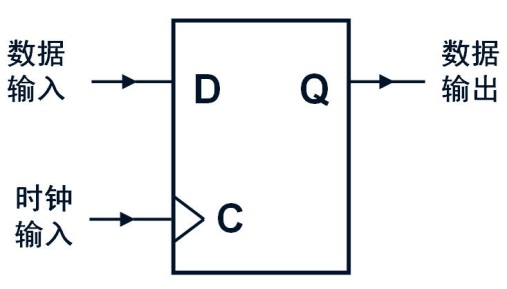
\includegraphics{media/image2.jpeg}
\caption{This is the caption}\label{fig:figure0}
}
\end{figure}

(source)

\begin{Shaded}
\begin{Highlighting}[]
\AlertTok{![This is the caption](media/image2.jpeg)}\NormalTok{\{\#fig:figure0\}}
\end{Highlighting}
\end{Shaded}
\end{frame}

\begin{frame}[fragile]{Figures (cont'd)}
\protect\hypertarget{sec:figures-contd}{}
If you just want a regular inline image, just make sure it is not the
only thing in the paragraph. One way to do this is to insert a
nonbreaking space after the image:

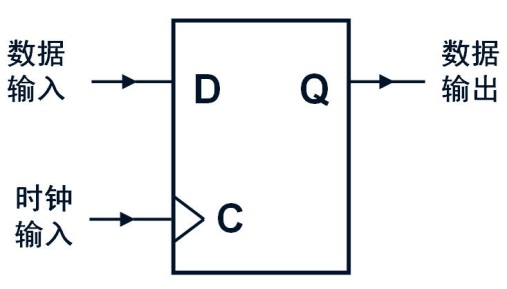
\includegraphics{media/image2.jpeg}\\

(source)

\begin{Shaded}
\begin{Highlighting}[]
\AlertTok{![No caption](media/image2.jpeg)}\NormalTok{\textbackslash{}}
\end{Highlighting}
\end{Shaded}
\end{frame}

\begin{frame}[fragile]{Render Diagrams using Tikz}
\protect\hypertarget{sec:render-diagrams-using-tikz}{}
\begin{columns}
\column{0.4\textwidth}

\scriptsize

\begin{Shaded}
\begin{Highlighting}[]
\KeywordTok{\textbackslash{}begin}\NormalTok{\{}\ExtensionTok{figure}\NormalTok{\}[hp]}
\FunctionTok{\textbackslash{}centering}
\FunctionTok{\textbackslash{}input}\NormalTok{\{pole2polar.tikz\}}
\FunctionTok{\textbackslash{}caption}\NormalTok{\{Example of constructing}
\NormalTok{    the polar of a point\}}\CommentTok{\%}
\KeywordTok{\textbackslash{}label}\NormalTok{\{}\ExtensionTok{fig:pole2polar}\NormalTok{\}}
\KeywordTok{\textbackslash{}end}\NormalTok{\{}\ExtensionTok{figure}\NormalTok{\}}
\end{Highlighting}
\end{Shaded}

\column{0.6\textwidth}

\begin{figure}[hp]
\centering
\definecolor{uuuuuu}{rgb}{0.26666666666666666,0.26666666666666666,0.26666666666666666}
\definecolor{ffqqqq}{rgb}{1.,0.,0.}
\definecolor{qqqqff}{rgb}{0.,0.,1.}
\definecolor{cqcqcq}{rgb}{0.7529411764705882,0.7529411764705882,0.7529411764705882}
\begin{tikzpicture}[scale=0.5,line cap=round,line join=round,>=triangle 45,x=1.0cm,y=1.0cm]
\draw [color=cqcqcq,, xstep=1.0cm,ystep=1.0cm] (-4.3,-6.2) grid (12.42,6.3);
\clip(-4.3,-6.2) rectangle (12.42,6.3);
\onslide<7->{
  \draw [rotate around={0.:(2.5,0.5)}] (2.5,0.5) ellipse (3.1024184114977142cm and 2.533114025595111cm);
}
\onslide<9->{
  \draw [domain=-4.3:12.42] plot(\x,{(-30.--3.*\x)/-7.});
}
\onslide<11->{
  \draw [domain=-4.3:12.42] plot(\x,{(--10.-1.*\x)/-10.});
}
\onslide<13->{
  \draw [domain=-4.3:12.42] plot(\x,{(-14.306522167487685--2.7190541871921186*\x)/-0.6334581280788179});
}
\onslide<14->{
  \draw [domain=-4.3:12.42] plot(\x,{(-3.--4.*\x)/3.});
}
\onslide<16->{
  \draw [domain=-4.3:12.42] plot(\x,{(--4.736-3.256*\x)/-4.736});
}
\onslide<17->{
  \draw [domain=-4.3:12.42] plot(\x,{(-17.497536945812808--3.4630541871921183*\x)/-2.3694581280788176});
}
\onslide<19->{
  \draw [color=ffqqqq,domain=-4.3:12.42] plot(\x,{(--10.85435667986003-2.9074169678196515*\x)/-0.2907416967819647});
}
\begin{scriptsize}
\onslide<3->{
  \draw [fill=qqqqff] (3.,3.) circle (2.5pt);
}
\onslide<3->{
  \draw[color=qqqqff] (3.14,3.36) node {$B$};
}
\onslide<6->{
  \draw [fill=qqqqff] (0.,-1.) circle (2.5pt);
}
\onslide<6->{
  \draw[color=qqqqff] (0.14,-0.64) node {$E$};
}
\onslide<7->{
  \draw[color=black] (1.,2.42) node {$c$};
}
\onslide<8->{
  \draw [fill=ffqqqq] (10.,0.) circle (2.5pt);
}
\onslide<8->{
  \draw[color=ffqqqq] (10.14,0.36) node {$F$};
}
\onslide<9->{
  \draw[color=black] (-4.14,5.9) node {$f$};
}
\onslide<10->{
  \draw [fill=uuuuuu] (4.736,2.256) circle (1.5pt);
}
\onslide<10->{
  \draw[color=uuuuuu] (4.88,2.54) node {$G$};
}
\onslide<11->{
  \draw[color=black] (12.18,0.08) node {$g$};
}
\onslide<12->{
  \draw [fill=uuuuuu] (5.369458128078818,-0.4630541871921182) circle (1.5pt);
}
\onslide<12->{
  \draw[color=uuuuuu] (5.5,-0.18) node {$H$};
}
\onslide<13->{
  \draw[color=black] (4.04,6.16) node {$h$};
}
\onslide<14->{
  \draw[color=black] (5.04,6.16) node {$i$};
}
\onslide<15->{
  \draw [fill=uuuuuu] (4.192307692307692,4.5897435897435885) circle (1.5pt);
}
\onslide<15->{
  \draw[color=uuuuuu] (4.34,4.86) node {$I$};
}
\onslide<16->{
  \draw[color=black] (-4.14,-3.48) node {$j$};
}
\onslide<17->{
  \draw[color=black] (8.9,-5.94) node {$k$};
}
\onslide<18->{
  \draw [fill=uuuuuu] (3.901565995525727,1.6823266219239372) circle (1.5pt);
}
\onslide<18->{
  \draw[color=uuuuuu] (4.04,1.96) node {$J$};
}
\onslide<19->{
  \draw[color=ffqqqq] (4.08,6.16) node {$l$};
}
\end{scriptsize}
\end{tikzpicture}

\caption{Example of constructing
    the polar of a point}%
\label{fig:pole2polar}
\end{figure}

\end{columns}
\end{frame}

\begin{frame}[fragile]{Table}
\protect\hypertarget{sec:table}{}
Simple tables can be generated using Markdown.

\scriptsize

\begin{columns}
\column{0.5\textwidth}

\begin{Shaded}
\begin{Highlighting}[]
\NormalTok{| Costs        | 28nm      | 20nm        |}
\NormalTok{| {-}{-}{-}{-}{-}{-}{-}{-}{-}{-}{-}{-} | {-}{-}{-}{-}{-}{-}{-}{-}{-} | {-}{-}{-}{-}{-}{-}{-}{-}{-}{-}{-} |}
\NormalTok{| Fab Costs    | 3B        | 4B {-} 7B     |}
\NormalTok{| Process R\&D  | 1.2B      | 2.1B {-} 3B   |}
\NormalTok{| Mask Costs   | 2M {-} 3M   | 5M {-} 8M     |}
\NormalTok{| Design Costs | 50M {-} 90M | 120M {-} 500M |}

\NormalTok{: Fab, process, mask, and design}
\NormalTok{  costs \{\#tbl:fab\}}
\end{Highlighting}
\end{Shaded}

\column{0.5\textwidth}

\hypertarget{tbl:fab}{}
\begin{longtable}[]{@{}lll@{}}
\caption{\label{tbl:fab}Fab, process, mask, and design
costs}\tabularnewline
\toprule\noalign{}
Costs & 28nm & 20nm \\
\midrule\noalign{}
\endfirsthead
\toprule\noalign{}
Costs & 28nm & 20nm \\
\midrule\noalign{}
\endhead
Fab Costs & 3B & 4B - 7B \\
Process R\&D & 1.2B & 2.1B - 3B \\
Mask Costs & 2M - 3M & 5M - 8M \\
Design Costs & 50M - 90M & 120M - 500M \\
\bottomrule\noalign{}
\end{longtable}

\end{columns}
\end{frame}

\hypertarget{sec:pandoc-crossref-filter}{%
\section{\texorpdfstring{\texttt{pandoc-crossref}
filter}{pandoc-crossref filter}}\label{sec:pandoc-crossref-filter}}

\begin{frame}[fragile]{\texttt{pandoc-crossref} filter}
\protect\hypertarget{sec:pandoc-crossref-filter-1}{}
With this filter, you can cross-reference figures (see
\cref{fig:figure0} and Fig. \ref{fig:pole2polar}), display equations
(see \cref{eq:semidef}), tables (see \cref{tbl:fab}) and sections
\cref{sec:intro}, \cref{sec:pandocx}

There is also support for code blocks, for example,
\cref{lst:captionAttr,lst:tableCaption}.

To compile:

\begin{Shaded}
\begin{Highlighting}[]
\ExtensionTok{$}\NormalTok{ pandoc }\AttributeTok{{-}F}\NormalTok{ pandoc{-}crossref }\AttributeTok{{-}t}\NormalTok{ beamer beamer.yaml }\DataTypeTok{\textbackslash{}}
\NormalTok{  crossref.yaml beamer.md }\AttributeTok{{-}o}\NormalTok{ intro.pdf}
\end{Highlighting}
\end{Shaded}
\end{frame}

\begin{frame}[fragile]{A sample \texttt{crossref.yaml}}
\protect\hypertarget{sec:a-sample-crossref.yaml}{}
\scriptsize

\begin{Shaded}
\begin{Highlighting}[]
\PreprocessorTok{{-}{-}{-}}
\FunctionTok{cref}\KeywordTok{:}\AttributeTok{ }\CharTok{True}
\FunctionTok{codeBlockCaptions}\KeywordTok{:}\AttributeTok{ }\CharTok{True}
\FunctionTok{lofTitle}\KeywordTok{:}\AttributeTok{ }\StringTok{"\#\# List of Figures"}
\FunctionTok{lotTitle}\KeywordTok{:}\AttributeTok{ }\StringTok{"\#\# List of Tables"}
\FunctionTok{autoSectionLabels}\KeywordTok{:}\AttributeTok{ }\CharTok{True}
\FunctionTok{figureTemplate}\KeywordTok{:}\AttributeTok{ $$t$$}
\FunctionTok{tableTemplate}\KeywordTok{:}\AttributeTok{ $$t$$}
\FunctionTok{figPrefix}\KeywordTok{:}
\AttributeTok{  }\KeywordTok{{-}}\AttributeTok{ }\StringTok{"Fig."}
\FunctionTok{eqnPrefix}\KeywordTok{:}
\AttributeTok{  }\KeywordTok{{-}}\AttributeTok{ }\StringTok{"Eq."}
\FunctionTok{tblPrefix}\KeywordTok{:}
\AttributeTok{  }\KeywordTok{{-}}\AttributeTok{ }\StringTok{"Table"}
\FunctionTok{lstPrefix}\KeywordTok{:}
\AttributeTok{  }\KeywordTok{{-}}\AttributeTok{ }\StringTok{"Listing"}
\FunctionTok{secPrefix}\KeywordTok{:}
\AttributeTok{  }\KeywordTok{{-}}\AttributeTok{ }\StringTok{"§"}
\CommentTok{...}
\end{Highlighting}
\end{Shaded}
\end{frame}

\begin{frame}[fragile]{Code blocks}
\protect\hypertarget{sec:code-blocks}{}
There are a couple options for code block labels. Those work only if
code block id starts with \texttt{lst:}, e.g.~\texttt{\{\#lst:label\}}
\end{frame}

\begin{frame}[fragile]{\texttt{caption} attribute}
\protect\hypertarget{sec:caption-attribute}{}
\texttt{caption} attribute will be treated as code block caption. If
code block has both id and \texttt{caption} attributes, it will be
treated as numbered code block.

\begin{Shaded}
\begin{Highlighting}[]
\OtherTok{main ::} \DataTypeTok{IO}\NormalTok{ ()}
\NormalTok{main }\OtherTok{=} \FunctionTok{putStrLn} \StringTok{"Hello World!"}
\end{Highlighting}
\end{Shaded}

(source)

\begin{Shaded}
\begin{Highlighting}[]
\NormalTok{\{\#lst:captionAttr .haskell caption="Listing caption A"\}}
\end{Highlighting}
\end{Shaded}
\end{frame}

\begin{frame}[fragile]{Table-style captions}
\protect\hypertarget{sec:table-style-captions}{}
Enabled with \texttt{codeBlockCaptions} metadata option. If code block
is immediately adjacent to paragraph, starting with \texttt{Listing:} or
\texttt{:}, said paragraph will be treated as code block caption.

Listing: Listing caption B

\begin{Shaded}
\begin{Highlighting}[]
\OtherTok{main ::} \DataTypeTok{IO}\NormalTok{ ()}
\NormalTok{main }\OtherTok{=} \FunctionTok{putStrLn} \StringTok{"Hello World!"}
\end{Highlighting}
\end{Shaded}
\end{frame}

\hypertarget{sec:pandoc-citeproc-filter}{%
\section{\texorpdfstring{\texttt{pandoc-citeproc}
filter}{pandoc-citeproc filter}}\label{sec:pandoc-citeproc-filter}}

\begin{frame}[fragile]{Bibliography}
\protect\hypertarget{sec:bibliography}{}
\begin{itemize}
\tightlist
\item
  See Aalst, Weijters, and Maruster
  (\protect\hyperlink{ref-Aalst-etal_2004}{2004}), or
\item
  See (\protect\hyperlink{ref-Baldi-etal_2008}{Baldi et al. 2008};
  \protect\hyperlink{ref-Canfora-Cerulo_2005a}{Canfora and Cerulo
  2005}).
\end{itemize}

(source)

\begin{Shaded}
\begin{Highlighting}[]
\SpecialStringTok{{-} }\NormalTok{See @Aalst{-}etal\_2004, or}
\SpecialStringTok{{-} }\NormalTok{See }\CommentTok{[}\OtherTok{@Baldi{-}etal\_2008;@Canfora{-}Cerulo\_2005a}\CommentTok{]}\NormalTok{.}
\end{Highlighting}
\end{Shaded}

To compile:

\begin{Shaded}
\begin{Highlighting}[]
\ExtensionTok{$}\NormalTok{ pandoc }\AttributeTok{{-}F}\NormalTok{ pandoc{-}crossref }\AttributeTok{{-}{-}citeproc} \AttributeTok{{-}t}\NormalTok{ beamer }\DataTypeTok{\textbackslash{}}
\NormalTok{  beamer.yaml crossref.yaml beamer.md }\AttributeTok{{-}o}\NormalTok{ intro.pdf}
\end{Highlighting}
\end{Shaded}
\end{frame}

\begin{frame}[allowframebreaks]{References}
\protect\hypertarget{sec:references}{}
\hypertarget{refs}{}
\begin{CSLReferences}{1}{0}
\leavevmode\vadjust pre{\hypertarget{ref-Aalst-etal_2004}{}}%
Aalst, W. van der, T. Weijters, and L. Maruster. 2004. {``Workflow
Mining: Discovering Process Models from Event Logs.''} \emph{IEEE
Transactions on Knowledge and Data Engineering} 16 (9): 1128--42.
\url{https://doi.org/10.1109/TKDE.2004.47}.

\leavevmode\vadjust pre{\hypertarget{ref-Baldi-etal_2008}{}}%
Baldi, Pierre F, Cristina V Lopes, Erik J Linstead, and Sushil K
Bajracharya. 2008. {``A Theory of Aspects as Latent Topics.''} In
\emph{ACM Sigplan Notices}, 43:543--62. 10. ACM.
\url{https://doi.org/10.1145/1449955.1449807}.

\leavevmode\vadjust pre{\hypertarget{ref-Canfora-Cerulo_2005a}{}}%
Canfora, G., and L. Cerulo. 2005. {``Impact Analysis by Mining Software
and Change Request Repositories.''} In \emph{11th IEEE International
Software Metrics Symposium (METRICS'05)}, 29. Como, Italy: IEEE.
\url{https://doi.org/10.1109/METRICS.2005.28}.

\end{CSLReferences}
\end{frame}

\end{document}
